\documentclass{article}

% Layout
\usepackage[a4paper,margin=2.5cm]{geometry}
\parindent=0pt
\frenchspacing

% Packages
\usepackage[none]{hyphenat}
\usepackage[english]{babel}
\usepackage{parskip}
\usepackage{hyperref}
\usepackage[backend=bibtex, sorting=none]{biblatex}
\usepackage{booktabs}
\usepackage{graphicx}

% Bibliography configuration
\DeclareFieldFormat[article, online]{title}{\emph{#1}} 
\bibliography{Report.bib}

% Hyperlink configuration
\hypersetup{colorlinks,linkcolor=black,citecolor=black,filecolor=black,urlcolor=black}

% Document contents
\begin{document}

\title{Distributed sentiment analysis on GitHub commit comments}
\author{Leon Helwerda (s1034375) and Tim van der Meij (s1115731)}
\date{\today}
\maketitle

\begin{abstract}
  In this report we discuss performing sentiment analysis on GitHub commit
  comments. We describe the problems and solutions related to downloading and
  preprocessing the dataset and gaining insights into the data using a naive
  implementation that uses lists with positive and negative words. After
  manually labeling 2000~training examples, we benchmark several classification
  algorithms and we use the most promising classifier in our final
  implementation where we apply the trained classifier on the entire dataset.
  We visualize the overall sentiment per programming language to show the
  potential of our approach. Distributing workload is key when working with 
  such a large dataset. Therefore, getting the data, preprocessing it and 
  performing the sentiment analysis is all done in a distributed manner with 
  help of OpenMPI and MapReduce.
\end{abstract}

\section{Introduction}\label{sec:introduction}
Sentiment analysis is a technique that aims to extract subjective information
from text, audio or other multimedia. This information contains, but is not
limited to, judgements or emotions on a certain topic. Sentiment analysis is
often troubled by the limitations of natural language processing and by the
large amounts of data available. Furthermore, in order to process all samples 
from a given dataset, we require that the sentiment analysis on one sample must 
be fast. Otherwise, the process quickly becomes infeasible and unsuitable for a
huge dataset.

In this report we focus only on sentiment analysis of textual content. We 
specifically use the GitHub commit comments dataset for our analysis. GitHub is 
an online platform that provides source code hosting and collaboration for both 
open-source and closed-source projects that use the Git version control system. 
When developing source code in a version-controlled environment, it is common 
practice to divide the implementation of functionality into \emph{commits}, 
which are small packages of code. Once the developer is ready to have the code 
reviewed, then reviewers can look at these commits and comment on them. For 
instance, a reviewer could add a comment to a specific line of code and suggest 
an improvement.

The GitHub commit comments dataset that we use consists of exactly these 
comments. The commit comments are particularly interesting, since developers 
and reviewers tend to put a lot of personal feelings in them. These emotions 
can range from happiness, when a commit is of high quality, to sadness or 
angriness when a commit is of poor quality.

We perform the sentiment analysis in a distributed manner. Since the total 
GitHub commit comments dataset is very large, and speed and efficiency are 
a concern, we aim to distribute most of the workload, including downloading and 
preprocessing data, over several worker nodes. We first implement a naive 
algorithm to get insights into the dataset and then apply those insights to the 
final implementation that uses a classifier to quickly classify commit comments 
as being positive, negative or neutral. Furthermore, we link the commit 
comments to the main programming language used in the code repository to be 
able to get insights into the sentiments of the developers per language.

Section~\ref{sec:problem} describes the research question in more detail as well
as give definitions of the techniques that we evaluate and related work. The
used dataset and the implementation of the distributed sentiment analysis
framework are discussed in Section~\ref{sec:dataset} and
Section~\ref{sec:implementation}, respectively. We present our experiments in
Section~\ref{sec:experiments} and discuss the results of the experiments in
Section~\ref{sec:results}. We list future research and conclude our analysis in
Section~\ref{sec:conclusion}.

\section{Problem statement}\label{sec:problem}
The goal of this research is to determine how we can perform sentiment analysis
on a large dataset in a distributed manner. In order to investigate this, we
develop a complete sentiment analysis framework in Python that contains all
techniques discussed in this report. The implementation is further outlined in 
Section~\ref{sec:implementation}.

Sentiment analysis allows for the retrieval of subjective information, such as
opinions, judgements or emotions, from text or other multimedia. Several types
of sentiment analysis exist, but the most used are classification of content
into an emotion category (`happy', `angry', `disappointed', et cetera) or
classification of content as being positive, negative or neutral. Since
sentiment analysis through the use of classification yields a probability score
for all categories, we are also able to numerically compare the sentiment in
different content, making it possible to determine if one piece of text is more
positive than another, for example. Our research focusses on performing 
sentiment analysis on textual content and classifying the textual content as 
being positive, negative or neutral.

Being able to automatically classify content into fixed categories can yield
previously unknown insights. Because of this, sentiment analysis is becoming
increasingly important for companies all over the world that want to know how
users review their products or services. For instance, web shops like Amazon
are interested in determining which products reviewers are positive about.
With this information Amazon might decide to recommend those products over
products with less positive reviews, thereby increasing customer satisfaction
and revenues. Users on a discussion platform can also benefit from sentiment 
analysis in order to detect whether a certain discussion has a positive or 
negative atmosphere.

Sentiment analysis is troubled by the limitations of natural language processing
as well as by the large amounts of available data. Natural language processing
limitations include, but are not limited to, making proper use of context and
detecting sarcasm. On top of that, sentiment analysis on a single text should be
fast in order to make working with a large dataset feasible.

% TODO: Perhaps split up in subsections?
% Perhaps also mention: "How do we obtain the dataset and preprocess it?"
% And: "How can we distribute the work onto worker nodes?" From presentation.
We propose a framework that performs sentiment analysis on large datasets in a
distributed manner. We aim to distribute most operations performed by the 
framework, such as downloading and preprocessing individual data dumps and
classification. We utilize the resources of the Distributed ASCI 
Supercomputer~3 (DAS-3) at the LIACS institute of Leiden University. The DAS-3 
has a total of 32~worker nodes consisting of commodity hardware and a number of 
hard drives, including a RAID configuration. A key feature of the framework is 
the distribution of workload over multiple worker nodes, or even over multiple 
processes on a single node. This provides a great speed-up when processing the 
large datasets that we use, of which more details are given in 
Section~\ref{sec:dataset}.

We implement two different approaches for performing sentiment analysis. The
first approach is the word list approach. Given a piece of text, we split the 
text into individual words and for each word we test if the word appears in 
fixed lists of positive and negative words. We count the number of positive and 
negative words in the text and perform a majority vote for the final 
classification of positive, negative or neutral. This is a basic approach that 
is expected to perform reasonably well, but at the same time we foresee issues 
with this approach.

For instance, when this naive analyzer encounters the word `good', the 
algorithm treats that word as positive, but if that word is preceded by the 
word `not', then the meaning is actually negative. The algorithm, because of 
its simplicity, is not able to distinguish these cases, and may end up deciding 
that the text is neutral. This shows the main problem of this approach: because 
we only look at individual words, we omit the context in which these words 
appear.

To overcome these issues and to actually take context into account, we implement
a second approach that uses a classifier to do the classification. With this
approach we do not need any fixed word lists. The classifier learns what
positive, negative and neutral texts are from training examples. There are two
main difficulties for this approach, namely that there is no labeled training
set available for the dataset we use. Secondly, it is not clear which 
classifier would be the best fit for the data. We therefore start by manually 
labeling 2000~commit comments as positive, negative or neutral.

Once we have a training set, we can train many different classifiers, such as 
a random forest classifier or a Gaussian naive Bayes classifier, and perform 
five-fold cross-validation. The resulting accuracies from the cross-validation 
allow us to get an idea of which classifier is the best fit for the data. After 
having trained the best classifier with the training set, we treat the data 
that has not been used for the training set as the test set. We provide the 
test set to the classifier and let the classifier put positive, negative or 
neutral labels on the commit comments based on learned information from the 
training phase.

In order to show the potential of the latter approach, we supplement each 
commit comment with the main programming language of the repository it belongs 
to. We perform sentiment analysis on the test data and with the resulting 
labels for each commit comment we visualize the distribution of positive and 
negative commit comments per programming language. This is done in order to 
obtain insight into the sentiment of developers that use different programming 
languages. It is not hard to imagine that the results of sentiment analysis on 
this dataset can be used to obtain many more interesting insights.

\subsection{Related work}\label{sec:related-work}
There are many papers and studies related to sentiment analysis, particularly 
on sentiment scores of small pieces of text. Such studies for example 
investigate the classification of sentiments of a Twitter data 
set~\cite{agarwal2011twitter,kouloumpis2011twitter}, or perform sentiment 
analysis on movie review comments~\cite{yessenov2009sentiment}. Often, the 
empirical studies provide techniques for classifying a specific corpus and 
compare these with general classifier approaches. Often, the novel techniques 
require a lot of tuning in order to make use of the features in the dataset as 
much as possible.

There are also studies related to sentiment analysis of the GitHub commit 
comments dataset, which we use in our 
analysis~\cite{guzman2014github,pletea2014security}. Again, these studies often 
provide a specific sentiment analysis tool which uses lexical extraction based 
on heuristics. An experiment with a very large dataset and with numerous 
classifier variants is often unavailable. There is one analysis of a large 
collection of GitHub commit messages which counts the number of messages that 
fall in one sentiment category and compares languages in this 
way~\cite{geeksta}. The downside of this approach is the use of a fixed word 
list which might not catch all messages and could incorrectly classify some 
messages as happy which are in fact not happy, for example.

\section{Dataset}\label{sec:dataset}
We use the GitHub commit comments dataset for our analysis. As described in the
introduction in Section~\ref{sec:introduction}, the GitHub commit comments
dataset contains comments that reviewers have attached to specific lines of
a Git commit or to an entire Git commit.

The dataset is provided by the GHTorrent 
project~\cite{ghtorrent,gousi2013ghtorrent}, which
publishes incremental and categorized dumps of data from the publicly
available GitHub API\@. We only use the commit comment dumps and the
repository dumps for our analysis, but, among others, issue comments, pull
request comments and events are also available. Every two months a new
incremental dump is published.

We focus on two types of dumps we use for our analysis, which are the
commit comments and repository dumps. The former is used for the sentiment
analysis itself, while the latter is used to assign to a commit the main 
programming language of the repository that it belongs to, which is useful for 
one of the experiments described in Section~\ref{sec:experiments}.

Each dump contains a part of the dataset, since GHTorrent generates incremental 
dumps on a bimonthly basis. A dump consists of one BSON file, which is 
a binary-encoded JSON file that is used for storing and exchanging data in 
a structured manner. The BSON file is converted to JSON and preprocessed, after 
which we obtain a file containing objects of the following form:

\begin{verbatim}
{
  "id": 8771097,
  "body": "It seems e.offsetX is not the way to get the relative cursor position
           in Firefox. I'm getting `undefined' in my experiments there.",
  "url": "https://api.github.com/repos/fedwiki/wiki-plugin-method/comments/8771097"
}
\end{verbatim}

We use the {\tt id} field as a unique identifier for cross-reference and
the {\tt body} field which contains the actual commit message. For the
experiments we also use the {\tt url} field to extract the name of the
repository that the commit belongs to in order to assign the main
programming language of that repository to the commit message.

The repositories dump is very similar, however, from that dump we only
extract the {\tt full\_name} field which contains the repository name and
the {\tt language} field which contains the main programming language used
in the repository.

The characteristics of both datasets (commit comments and repositories) are
listed in Table~\ref{tab:dataset}. We list details of the 2015--01--29
commit comments dump as that dump has been used for manually labeling commit
comments to create a training set, which we discuss in
Section~\ref{sec:implementation}. Furthermore, we list details of the
2015--01--29 commit comments dump when all comments with non-Latin characters
(Chinese, Russian, et cetera) have been removed. Those comments are not
relevant for our research as we only focus on English commit comments. Finally
we list the details for all commit comment dumps and all repository dumps. In
the table, `preprocessed' indicates that we have applied our preprocessor to
remove unneeded fields for our research.

\begin{table}[h]
  \centering
  \begin{tabular}{l r l}
    \toprule
    \textbf{Dump}                           & \textbf{\# items} & \textbf{Size}                           \\
    \midrule
    2015--01--29 commit comments            & 182.282           & 43~MB compressed, 267~MB uncompressed   \\
    2015--01--29 Latin-only commit comments & 165.427           & 42~MB preprocessed                      \\
    Commit comments (17 dumps)              & 1.731.251         & 434~MB compressed                       \\
    Repositories (17 dumps)                 & 12.802.797        & 10.8~GB compressed, 1.3~GB preprocessed \\
    \bottomrule
  \end{tabular}
  \caption{Characteristics of the GitHub commit comment and repository datasets.}\label{tab:dataset}
\end{table}

\section{Implementation}\label{sec:implementation}
Our implementation consists of a number of components that can interact with 
each other. Among others, we have implemented a preprocessor component for 
extracting the datasets described in Section~\ref{sec:dataset}, an analyzer and 
classifier that can generate predictions for sentiment scores, a plotting 
framework, an experiment runner and an interactive dataset labeler.

We implemented these tools using the Python programming language with 
distributed processing in mind. The components for making predictions and 
counting frequencies can be automatically distributed using MapReduce and the 
preprocessor and some parts of the toolchain can be parallelized using MPI, as 
described in more detail in Section~\ref{sec:mpi}.

Many parts of the toolchain use the notion of \emph{groups} in order to make 
analysis possible for different goals. For example, one can group the commit 
comments on their {\tt id}, which allows for visual output of the predictions 
and cross-referencing the results. The use of the {\tt score} group allows the 
reducer in Section~\ref{sec:reducer} to count the frequencies of each score, 
which can then be visualized with a frequency plot. Other groups function more 
like creating partitions of the dataset. The groups play an important role in
the filtering phase of the preprocessor from Section~\ref{sec:preprocessor},
and the plotter can also create different plots for groups, such as the
{\tt algo} group for the results of the experiment runner in
Section~\ref{sec:experiment-runner}.

\subsection{Preprocessor}\label{sec:preprocessor}
The preprocessor is the first step in the implementation. The dataset from 
Section~\ref{sec:dataset} consists of different types of dumps and is split 
into multiple incremental dumps that are generated bimonthly. Therefore, we 
need a tool to automatically perform the phases of downloading, extracting, 
converting, processing and filtering the dumps of GitHub data from the 
GHTorrent archives.

Firstly, we use a scraper that checks the downloads page of GHTorrent and 
creates a list of possible dumps to download. The preprocessor checks whether 
the dump file already exists and otherwise it downloads the compressed dump and 
extracts it. Afterwards, the extracted BSON file, a binary JSON format, is 
converted to JSON\@. At this point, we can filter fields depending on the 
type of dump.

The {\tt repos} dumps, containing the repositories dataset, are filtered on the 
{\tt language} field and stored in an efficient format. This format, called a
\emph{shelve}, is a key-value based storage which allows transparent reads and 
writes. This makes it possible to merge the shelves of each dump in order to 
obtain a full mapping from repository names to the main programming language of 
those repositories. We use this to augment the data from the commit comments
dataset for usage in the experiments in Section~\ref{sec:experiments}.

The dataset of main importance is based on the {\tt commit\_comments} dumps, 
which contain the comments that reviewers make on pieces of code and commits in 
specific repositories. These commit comments are well-suited for sentiment 
analysis due to the emotions that reviewers express about the code. We remove
commit comments that have non-ASCII Unicode characters in it, in order to
remove comments in foreign non-Latin languages. We focus our classification
tools on English comments.

We extract the relevant fields, namely the ID for cross-reference, the message 
body containing the textual content itself, and a group if provided. We extract 
the repository name from the given URL in the dataset. In case of the 
`language' group, we link this repository name to the main language that we 
extracted from the {\tt repos} dumps.

The preprocessor automatically performs the chosen task with interactive 
progress output on each step. This script can therefore extract data from the
{\tt repos} dumps and create a shelve of the languages of all repositories. The
{\tt commit\_comments} task filters the dumps in order to keep the necessary
fields relevant to the commit comments, including the group.

Note that the preprocessor can also be run using MPI in order to parallelize 
the phases for different dumps. We can distribute the workload across nodes, 
with a master that schedules a new task for processes that are done with one 
dump, achieving automatic load balancing. We describe the implementation of MPI 
in our tools in Section~\ref{sec:mpi}.

\subsection{Naive analyzer}\label{sec:analyzer}
We implement a naive approach as a baseline for comparing against real 
classifiers. Given a commit comment, we split the text into separate words and 
compare each word against two word lists, respectively containing positive and 
negative words. Depending on which word list the word appears in, the score of 
the entire message is updated. If the word is not in any word list, then it 
does not affect the score. We calculate the score as an average of all the 
scores of each word ($-1$ if negative or $1$ if positive) divided by the number 
of words in one of the lists.

After data inspection, the word lists are augmented with emoticons and smileys 
that are often used on GitHub in order to express emotions and opinions 
regarding the commit. We also use a script to check which words that are not 
in either word lists occur in commit comments with a certain score, in order to 
add more words that are relevant for the scores.

During the word splitting, we sanitize words by removing quotes and other 
non-alphanumeric characters. In order to handle emoticons correctly, we use 
a specialized regular expression that considers emoticons as individual words 
instead of splitting or sanitizing them.

The {\tt id} group gives colored output, while other groups are suitable for 
usage with the reducer, as explained in Section~\ref{sec:reducer}. The analyzer
can be run using MapReduce which we also explain in that section. One can then
use the plotter for further analysis, as outlined in Section~\ref{sec:plotter}.

\subsection{Classifier}\label{sec:classifier}
With the structure of the naive analyzer at hand, we implement a tool that can 
give similar output as the naive analyzer, but instead it uses a classifier to
predict the scores. The classifier tool can also perform other tasks such as 
cross-validation or saving a trained model.

The classifier tool can use one of the classifiers or regressors available in
the \textsc{scikit-learn} machine learning toolkit~\cite{scikit-learn}. The tool
creates the model and trains it using the labeled training set that we created
with the labeler from Section~\ref{sec:labeler}. The trained model can then be
stored as a serialized \emph{pickle} file, which is a binary format readable by
Python programs. The model file can then be distributed to worker nodes, or one
can use it to predict the scores for a given commit comments dataset immediately.
Figure~\ref{fig:classifier-output} shows visual output of the classifier tool.

\begin{figure}[h!]
  \centering
  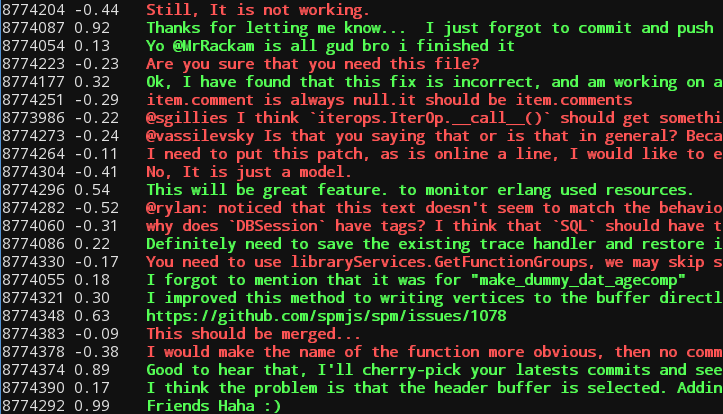
\includegraphics[width=0.5\textwidth]{Images/Classifier.png}
  \caption{Visual output of the classifier tool. Each line of the output
           consists of the ID, the sentiment score and the textual content of
           a commit comment. A negative score yields red text in the output,
           whereas a positive score yields green text in the
           output.}\label{fig:classifier-output}
\end{figure}

Another use of the tool is to cross-validate the chosen classifier. For a given 
number of folds, the labeled dataset is split into that number of folds, and 
the same number of models are created. Each model is trained with one fold and 
then the scores on the rest of the folds are predicted. We then compare these 
predictions with the actual labels of each comment, and calculate the average 
correctness of the models.

The predictions themselves can again be analyzed using the reducer and plotter, 
similar to the naive analyzer output. The classifier can therefore be run using 
MapReduce as well. When using the preprocessor with MPI to retrieve all commit 
comments dumps in a distributed way, one can also run the classifier to predict
the comments in the dumps on the worker nodes.

\subsection{MapReduce and reducer}\label{sec:reducer}
% TODO: Cite MapReduce/Hadoop
MapReduce is a component of Hadoop which allows to create two kinds of jobs: 
mappers and reducers. The mappers receive input on which they perform 
calculations and their output is sorted and split up to the reducer jobs, which 
can, for example, make counts or perform other aggregation tasks. This allows 
for distributed computation in phases.

We make use of MapReduce for our prediction and analysis tools. The naive 
analyzer from Section~\ref{sec:analyzer} and the classifier described in 
Section~\ref{sec:classifier} conform to the input and output requirements of 
a mapper. The output can be keyed by a certain group and the sorting can take 
into account which part is the key and which part is a value.

The combiner part of MapReduce performs the sorting, so that the output becomes 
suitable for the reducer. This script simply counts the frequency of a certain 
score in the file, and the output is then also sorted on those scores. In case 
of groups, the input is sorted on each group value first, thus the frequency
counts also happen per group and per score. This makes it possible to plot the
counts in a frequency plot or to visualize the relative scores of each group.
% TODO: Example

\subsection{Plotter}\label{sec:plotter}
\ldots

\subsection{Experiment runner}\label{sec:experiment-runner}
Determining the best classifier to use from the \textsc{scikit-learn} toolkit is
essential for obtaining reliable classifications. Since our labeled training
set containing 2000 labeled commit comments is relatively small, it is possible
to explore a large number of different classifiers with many different
combinations of parameters. We therefore develop an experiment runner that
performs cross-validation (five folds by default, but the number of folds is
configurable) on all classifiers and parameter combinations listed in a
manifest file.

The experiment runner, as mentioned before, depends on the availability of
a manifest file, which is a JSON file that contains an array of objects
describing the classifier and the parameters to test. An example entry
of the manifest file is the following:

\begin{verbatim}
{
  "class_name": "AdaBoostClassifier",
  "module": "sklearn.ensemble.weight_boosting",
  "name": "Ada Boost classifier",
  "parameters": {
    "n_estimators": [
      10,
      50,
      100,
      250,
      500
    ],
    "learning_rate": [
      0.1,
      0.2,
      0.3,
      0.4,
      0.5
    ]
  }
}
\end{verbatim}

In a manifest entry we mention the class name of the classifier to test, the
module to which the classifier belongs, the name of the classifier and the
parameters of the classifier that must be tested. In the example above, we have 
two parameters, namely {\tt n\_estimators} and
{\tt learning\_rate}. The manifest entry essentially indicates that we perform
cross-validation for the Ada Boost classifier with all possible combinations
of the parameter values. In this case we perform 25 runs, namely one with
{\tt n\_estimators = 10} and {\tt learning\_rate = 0.1}, one with
{\tt n\_estimators = 10} and {\tt learning\_rate = 0.2}, and so on.

We use a manifest file that contains 15 different classifiers. The
parameters and the values of the parameters to test have been determined by
studying the \textsc{scikit-learn} toolkit documentation. The experiment runner
reads the manifest file and performs cross-validation for each mentioned
classifier and for each parameter combination. The results of the
cross-validation are written to an output JSON file that the plotter from
Section~\ref{sec:plotter} can take as input and, using the `algo' group,
creates an SVG plot for each classifier.

Using the experiment runner on the training set gives an indication of
how accurate each classifier is on our dataset. The classifier and
parameter combination that yields the highest accuracy is used for the
final classifier.

\subsection{Labeler}\label{sec:labeler}
As a labeled training set does not yet exist for the GitHub commit comments
dataset, we have to make one ourselves. In order to streamline this process
and to collaborate on the effort, we implement a labeler. We use the commit
comments dump from 29--01--2015 to create our labeled training set.

The labeler loads this dataset, presents each commit comment individually to
the user, displays a prediction based on the naive word list approach and asks
the user whether or not he or she agrees with the prediction. If so, simply
pressing Enter stores the label for that commit comment. If not, the user
can enter `p' for positive, `n' for negative, `t' for neutral and `u' for
unknown, thereby overriding the prediction. We mark commit comments as unknown
such that the classifier ignores them if they do not contain useful content,
for instance comments containing only names of variables. We do not want to
confuse the classifier with those comments during the training phase to avoid
mispredictions.

In order to collaborate on the effort, the commit comments along with their
labels are stored in JSON format. The labeler automatically resumes where
the last collaborator left off. For example, if the first collaborated labeled
up until commit comment 500, then a second collaborator would resume labeling
at commit commit 501, thereby skipping already labeled commit comments. The
JSON file with the commit comment labels can therefore easily be put in a
version control system such that any user can use the labeler and continue 
where others left off.

\subsection{MPI}\label{sec:mpi}
% TODO: Explain preprocessor master/worker job dispatching and some about 
% classifier support
\ldots

\section{Experiments}\label{sec:experiments}
% TODO: Explain experiments: timing, memory?, analyzer/classifier frequency 
% plots?, algorithm comparisons, language sentiments
\ldots

\subsection{Results}\label{sec:results}
% TODO: Split up in sections? Perhaps combine experiments and results?
\ldots

\section{Conclusion}\label{sec:conclusion}
\ldots

\subsection{Future research}\label{sec:future-research}
% TODO: Other approaches: PCA and sentiments in more dimensions (categories), 
% extension to specific users/repos/communities/discussion (online live data 
% stream), comparison with other classifiers (neural networks, NLTK) and 
% specific interpretations of classifiers (RandomForest out of bag error).
\ldots

\section*{References}\label{sec:references}
\printbibliography[heading=none]

\section*{Appendix}
% TODO: Appendix (README, link to open-sourced repository)
\ldots

\end{document}
